\bivtask{Scan Conversion für Ellipsen}{10 = 6 + 1 + 3}
%
Die Standardellipse
\begin{center}
  %% Creator: Inkscape inkscape 0.91, www.inkscape.org
%% PDF/EPS/PS + LaTeX output extension by Johan Engelen, 2010
%% Accompanies image file 'ellipse1.pdf' (pdf, eps, ps)
%%
%% To include the image in your LaTeX document, write
%%   \input{<filename>.pdf_tex}
%%  instead of
%%   \includegraphics{<filename>.pdf}
%% To scale the image, write
%%   \def\svgwidth{<desired width>}
%%   \input{<filename>.pdf_tex}
%%  instead of
%%   \includegraphics[width=<desired width>]{<filename>.pdf}
%%
%% Images with a different path to the parent latex file can
%% be accessed with the `import' package (which may need to be
%% installed) using
%%   \usepackage{import}
%% in the preamble, and then including the image with
%%   \import{<path to file>}{<filename>.pdf_tex}
%% Alternatively, one can specify
%%   \graphicspath{{<path to file>/}}
%% 
%% For more information, please see info/svg-inkscape on CTAN:
%%   http://tug.ctan.org/tex-archive/info/svg-inkscape
%%
\begingroup%
  \makeatletter%
  \providecommand\color[2][]{%
    \errmessage{(Inkscape) Color is used for the text in Inkscape, but the package 'color.sty' is not loaded}%
    \renewcommand\color[2][]{}%
  }%
  \providecommand\transparent[1]{%
    \errmessage{(Inkscape) Transparency is used (non-zero) for the text in Inkscape, but the package 'transparent.sty' is not loaded}%
    \renewcommand\transparent[1]{}%
  }%
  \providecommand\rotatebox[2]{#2}%
  \ifx\svgwidth\undefined%
    \setlength{\unitlength}{297.33493182bp}%
    \ifx\svgscale\undefined%
      \relax%
    \else%
      \setlength{\unitlength}{\unitlength * \real{\svgscale}}%
    \fi%
  \else%
    \setlength{\unitlength}{\svgwidth}%
  \fi%
  \global\let\svgwidth\undefined%
  \global\let\svgscale\undefined%
  \makeatother%
  \begin{picture}(1,0.49511879)%
    \put(0,0){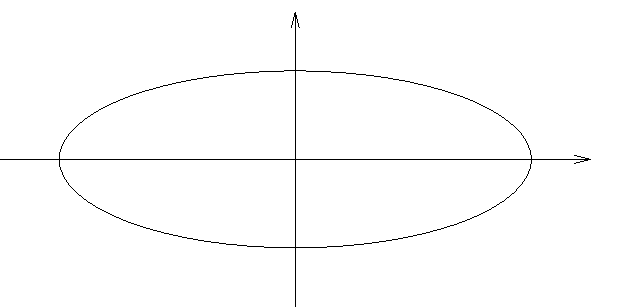
\includegraphics[width=\unitlength,page=1]{ellipse1.pdf}}%
    \put(0.48611848,0.40035657){\color[rgb]{0,0,0}\makebox(0,0)[lb]{\smash{$b$}}}%
    \put(0.04762306,0.20966254){\color[rgb]{0,0,0}\makebox(0,0)[lb]{\smash{$-a$}}}%
    \put(0.86750658,0.20966254){\color[rgb]{0,0,0}\makebox(0,0)[lb]{\smash{$a$}}}%
    \put(0.48611848,0.47663418){\color[rgb]{0,0,0}\makebox(0,0)[lb]{\smash{$y$}}}%
    \put(0.9629545,0.20966254){\color[rgb]{0,0,0}\makebox(0,0)[lb]{\smash{$x$}}}%
    \put(0.48611848,0.05730911){\color[rgb]{0,0,0}\makebox(0,0)[lb]{\smash{$-b$}}}%
  \end{picture}%
\endgroup%

\end{center}
mit Mittelpunkt im Punkt $(0, 0)$ und den Halbachsen $a$ und $b$ ist 
durch die Gleichung \[ F(x, y) = b² x² + a² y² - a² b² = 0 \] gegeben.

Der erste Quadrant muss nun in zwei Regionen aufgeteilt werden:
\begin{center}
  %% Creator: Inkscape inkscape 0.91, www.inkscape.org
%% PDF/EPS/PS + LaTeX output extension by Johan Engelen, 2010
%% Accompanies image file 'ellipse2.pdf' (pdf, eps, ps)
%%
%% To include the image in your LaTeX document, write
%%   \input{<filename>.pdf_tex}
%%  instead of
%%   \includegraphics{<filename>.pdf}
%% To scale the image, write
%%   \def\svgwidth{<desired width>}
%%   \input{<filename>.pdf_tex}
%%  instead of
%%   \includegraphics[width=<desired width>]{<filename>.pdf}
%%
%% Images with a different path to the parent latex file can
%% be accessed with the `import' package (which may need to be
%% installed) using
%%   \usepackage{import}
%% in the preamble, and then including the image with
%%   \import{<path to file>}{<filename>.pdf_tex}
%% Alternatively, one can specify
%%   \graphicspath{{<path to file>/}}
%% 
%% For more information, please see info/svg-inkscape on CTAN:
%%   http://tug.ctan.org/tex-archive/info/svg-inkscape
%%
\begingroup%
  \makeatletter%
  \providecommand\color[2][]{%
    \errmessage{(Inkscape) Color is used for the text in Inkscape, but the package 'color.sty' is not loaded}%
    \renewcommand\color[2][]{}%
  }%
  \providecommand\transparent[1]{%
    \errmessage{(Inkscape) Transparency is used (non-zero) for the text in Inkscape, but the package 'transparent.sty' is not loaded}%
    \renewcommand\transparent[1]{}%
  }%
  \providecommand\rotatebox[2]{#2}%
  \ifx\svgwidth\undefined%
    \setlength{\unitlength}{190.99073722bp}%
    \ifx\svgscale\undefined%
      \relax%
    \else%
      \setlength{\unitlength}{\unitlength * \real{\svgscale}}%
    \fi%
  \else%
    \setlength{\unitlength}{\svgwidth}%
  \fi%
  \global\let\svgwidth\undefined%
  \global\let\svgscale\undefined%
  \makeatother%
  \begin{picture}(1,0.45034525)%
    \put(0,0){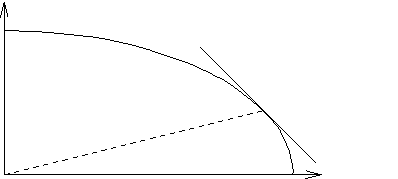
\includegraphics[width=\unitlength,page=1]{ellipse2.pdf}}%
    \put(0.06625593,0.23781583){\color[rgb]{0,0,0}\makebox(0,0)[lb]{\smash{Region 1}}}%
    \put(0.37224022,0.04446568){\color[rgb]{0,0,0}\makebox(0,0)[lb]{\smash{Region 2}}}%
    \put(0.56896632,0.29551397){\color[rgb]{0,0,0}\makebox(0,0)[lb]{\smash{Tangente mit Steigung $-1$}}}%
    \put(0.69295594,0.17981078){\color[rgb]{0,0,0}\makebox(0,0)[lb]{\smash{$(xᵣ, yᵣ)$}}}%
  \end{picture}%
\endgroup%
%ᵣ
\end{center}
Für den Punkt $(xᵣ, yᵣ)$, an dem die Tangente Steigung $-1$ hat, gilt die Bedingung
\[ a² yᵣ = b² xᵣ \,\text. \]%
\begin{bivsubt}
  \bivitem\label{it:ellScanConv} Formulieren Sie einen
    \emph{inkrementellen Scan-Conversion-Algorithmus} für Ellipsen. 
    Verwenden Sie zunächst für Region 1 eine Variable $d₁$ für die
    Entscheidung zwischen Ost und Südost. Am Übergang zu Region 2 muss 
    eine neue Variable $d₂$ initialisiert werden für die Wahl zwischen 
    Südost und Süd. (Ganzzahlige Rechnung ist hier nicht verlangt.)
  \bivitem\label{it:ellGanzZ} Wie könnte man den Algorithmus 
    modifizieren, damit ganzzahlig gerechnet werden kann?
  \bivitem\label{it:ellImpl} Implementieren Sie den Algorithmus aus
    Teil~\ref{it:ellScanConv} oder die modifizierte Variante aus
    Teil~\ref{it:ellGanzZ}, sofern Sie Teil~\ref{it:ellGanzZ}
    bearbeitet haben. Benutzen Sie eine Funktion namens 
    \texttt{drawEllipsePoints}, die zu einem Punkt zusätzlich die 
    anderen drei aus Symmetriegründen festgelegten Punkte zeichnet.
\end{bivsubt}

% Geben Sie Ihre Ausarbeitungen zu Teil~\ref{it:ellScanConv} und
% \ref{it:ellGanzZ} schriftlich ab. 
Ein Rahmenprogramm für die Implementierung in Teil~\ref{it:ellImpl} 
finden Sie im Verzeichnis \bivfolder{/home/bildgen/Aufgaben/ellipsen}.
